\section{Results}
\label{sec:results}

\subsection{Induction Scores Are Highly Correlated but Dramatically Different in Magnitude}
\label{sec:results_scores}

\Figref{fig:heatmaps} shows induction score heatmaps across all 144 heads (12 layers $\times$ 12 heads) on random and natural data.
The spatial pattern of which heads score highly is similar across conditions, but the scales differ by an order of magnitude: the maximum random score is 0.937 (L5.H1) while the maximum natural score is 0.082 (L6.H9).

\begin{figure}[t]
    \centering
    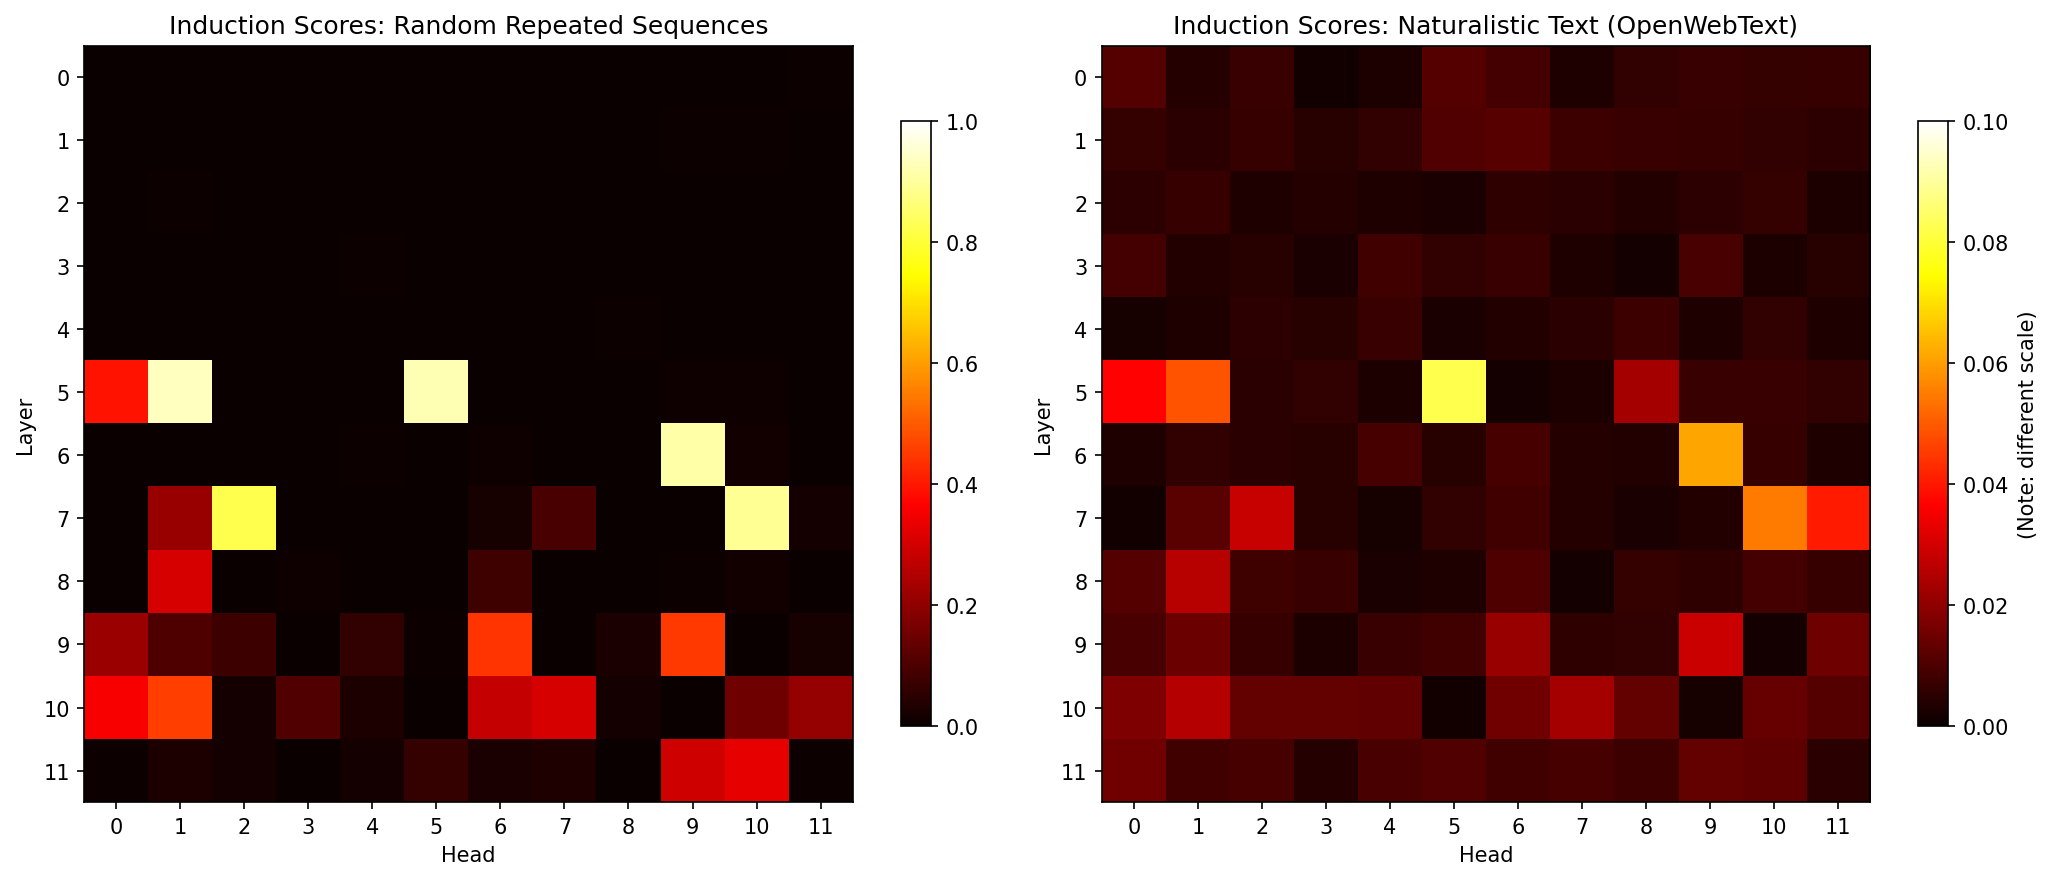
\includegraphics[width=0.95\linewidth]{figures/induction_heatmaps.png}
    \caption{Induction score heatmaps across all 144 attention heads in \gpttwo. \figleft Random repeated sequences (scale 0--1). \figright Natural text from \owt (scale 0--0.1). The same heads score highly in both conditions, but natural-text scores are $\sim$10$\times$ lower. Note the different color scales.}
    \label{fig:heatmaps}
\end{figure}

\Figref{fig:scatter} quantifies this relationship.
The Spearman rank correlation between random and natural induction scores is $\rho = 0.839$ ($p < 10^{-30}$), and the Pearson correlation is $r = 0.826$ ($p < 10^{-30}$).
All points fall well below the $y = x$ line, confirming that every head shows weaker induction behavior on natural text.

\begin{figure}[t]
    \centering
    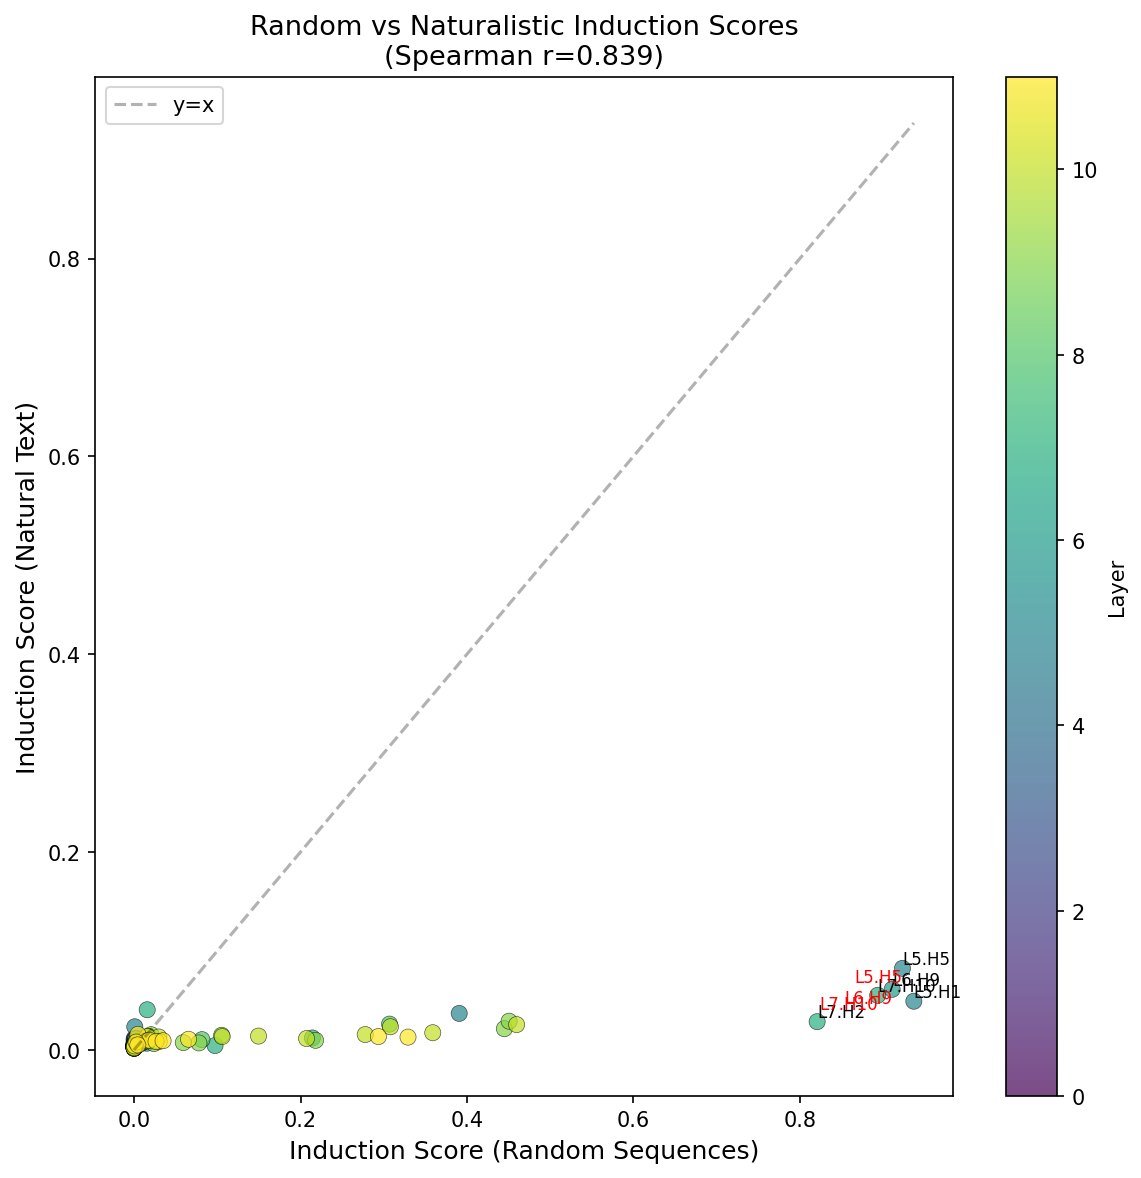
\includegraphics[width=0.65\linewidth]{figures/random_vs_natural_scatter.png}
    \caption{Scatter plot of induction scores on random ($x$-axis) vs.\ natural ($y$-axis) data for each of 144 heads. The strong correlation (Spearman $\rho = 0.84$) confirms that the same heads do induction in both conditions, while the distance from the $y = x$ line shows scores are 10--40$\times$ lower on natural text.}
    \label{fig:scatter}
\end{figure}

\Tabref{tab:top_heads} lists the top induction heads and their scores in both conditions.
The ratio between random and natural scores ranges from 11$\times$ to 40$\times$, with a median of 13$\times$ across the top five heads.

\begin{table}[t]
    \centering
    \caption{Top induction heads ranked by random-sequence score. Natural-text scores are 10--40$\times$ lower despite similar token repeat rates (50\% vs.\ 41\%). Best natural score in \textbf{bold}.}
    \label{tab:top_heads}
    \begin{tabular}{@{}lccc@{}}
        \toprule
        Head & Random $\iscore$ & Natural $\iscore$ & Ratio \\
        \midrule
        L5.H1  & 0.937 & 0.076 & 12.3$\times$ \\
        L6.H9  & 0.911 & \textbf{0.082} & 11.1$\times$ \\
        L7.H10 & 0.897 & 0.048 & 18.7$\times$ \\
        L7.H2  & 0.830 & 0.021 & 39.5$\times$ \\
        L5.H0  & 0.791 & 0.061 & 13.0$\times$ \\
        \bottomrule
    \end{tabular}
\end{table}

\para{Top-K overlap.}
We also measure the overlap between the $K$ highest-scoring heads in each condition (\tabref{tab:overlap}).
At $K = 5$, four of the top five heads are shared (80\% overlap), and at $K = 20$, fourteen are shared (70\%).
Critically, no head crosses the standard 0.10 induction threshold on natural text---the maximum natural score is 0.082---yielding zero ``universal'' induction heads and zero ``naturalistic-only'' induction heads under the standard definition.

\begin{table}[t]
    \centering
    \caption{Overlap between top-$K$ induction heads on random vs.\ natural data. High overlap confirms the same heads are identified in both conditions.}
    \label{tab:overlap}
    \begin{tabular}{@{}ccc@{}}
        \toprule
        $K$ & Shared Heads & Overlap (\%) \\
        \midrule
        5  & 4  & \textbf{80} \\
        10 & 7  & 70 \\
        20 & 14 & 70 \\
        \bottomrule
    \end{tabular}
\end{table}

\subsection{Fuzzy Matching Does Not Reveal Hidden Induction}
\label{sec:results_fuzzy}

One natural explanation for low naturalistic induction scores is that natural text requires \emph{fuzzy} matching---attending to semantically similar rather than identical prior tokens.
To test this, we computed fuzzy induction scores using cosine similarity $> 0.8$ between token embeddings.

The fuzzy scores are nearly identical to exact-match scores: the Spearman correlation between exact and fuzzy scores on natural text is $r = 0.990$, and the maximum fuzzy score (0.065) is actually \emph{lower} than the maximum exact score (0.082).
Relaxing the matching criterion does not reveal hidden induction behavior.
The bottleneck is not matching precision but rather that natural text provides many useful attention targets beyond the induction-pattern position.

\subsection{Late-Layer Heads Copy More on Natural Text}
\label{sec:results_copying}

While the induction score measures where heads attend (the QK circuit), the OV copying score measures what they do with that information.
\Figref{fig:copying} reveals a striking pattern: late-layer heads (layers 9--11) show dramatically higher copying scores on natural text than on random data, even as their induction attention patterns are weaker.

\begin{figure}[t]
    \centering
    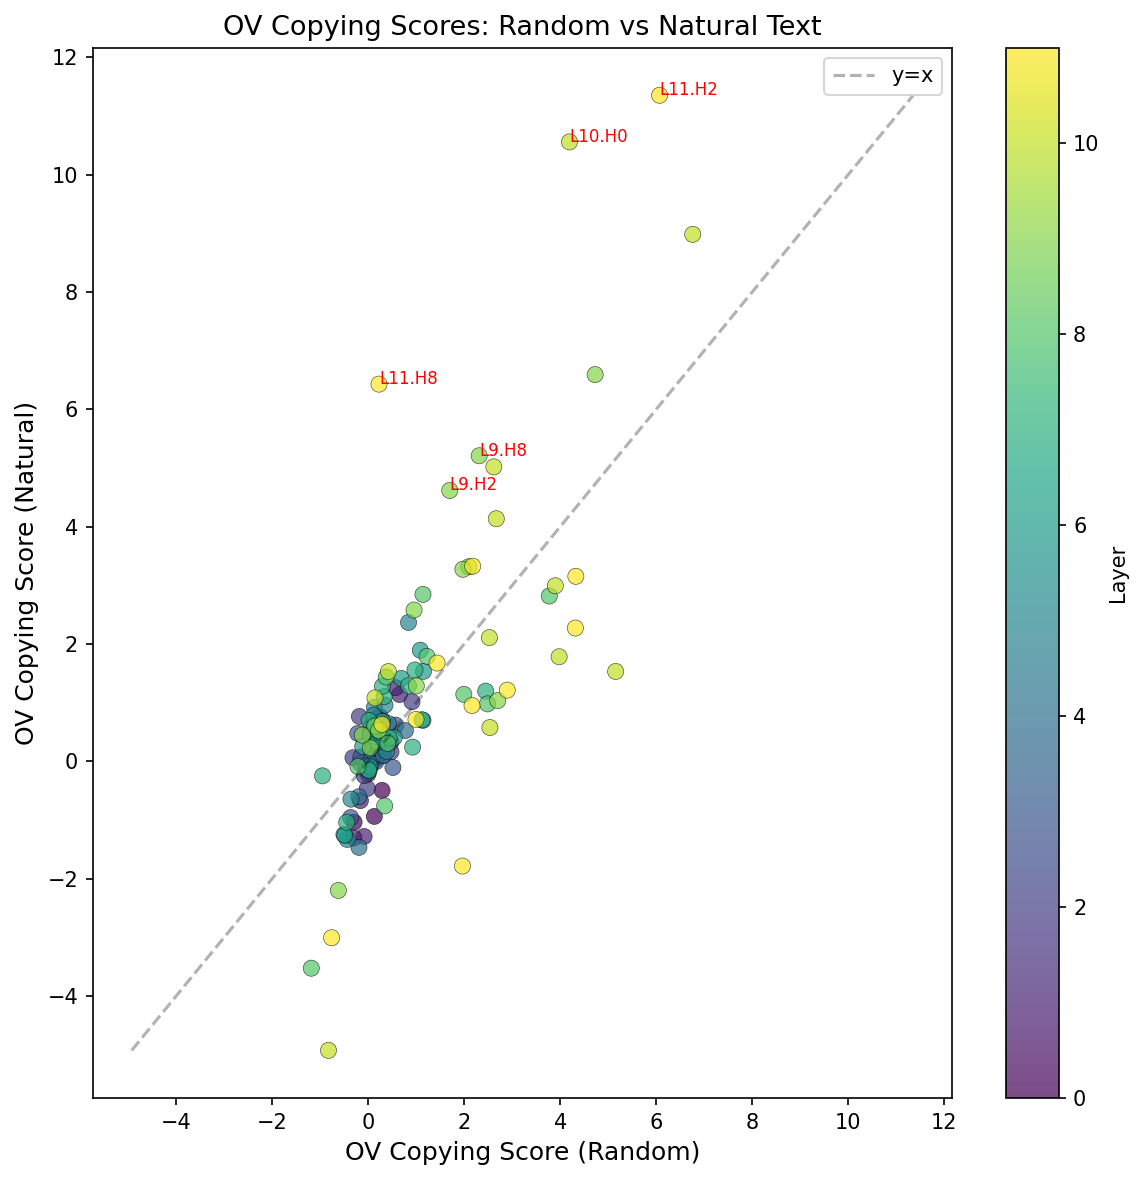
\includegraphics[width=0.65\linewidth]{figures/copying_scores_scatter.png}
    \caption{OV copying scores on random ($x$-axis) vs.\ natural ($y$-axis) data. Points above the diagonal indicate stronger copying on natural text. Late-layer heads (layers 9--11, warm colors) cluster above the diagonal, with L11.H8 showing a 29$\times$ increase on natural text.}
    \label{fig:copying}
\end{figure}

\Tabref{tab:copying} lists the heads with the largest naturalistic copying enrichment.
Head L11.H8 increases its copying score from 0.22 on random data to 6.43 on natural text---a 29$\times$ jump.
Head L10.H0 shows the largest absolute difference ($+6.37$).
These heads' OV circuits are tuned for natural language patterns in a way that random token distributions fail to activate.

\begin{table}[t]
    \centering
    \caption{Heads with the strongest naturalistic copying enrichment. Natural copying scores exceed random scores by 2--29$\times$ for late-layer heads, indicating distribution-sensitive OV circuits. Largest difference in \textbf{bold}.}
    \label{tab:copying}
    \begin{tabular}{@{}lccc@{}}
        \toprule
        Head & Natural $\cscore$ & Random $\cscore$ & Difference \\
        \midrule
        L10.H0 & 10.56 & 4.19 & \textbf{+6.37} \\
        L11.H8 & 6.43  & 0.22 & +6.20 \\
        L11.H2 & 11.35 & 6.07 & +5.28 \\
        L9.H2  & 4.62  & 1.70 & +2.92 \\
        L9.H8  & 5.21  & 2.31 & +2.90 \\
        \bottomrule
    \end{tabular}
\end{table}

\Figref{fig:layer} provides a layer-wise summary.
Induction scores diverge sharply between conditions in layers 5--11 (random $\gg$ natural), while copying scores converge and even reverse in late layers (natural $>$ random).
Attention entropy is similar across conditions, suggesting that the difference is not driven by more diffuse attention on natural text overall, but rather by a reallocation of attention away from the specific induction-pattern position to other contextually relevant positions.

\begin{figure}[t]
    \centering
    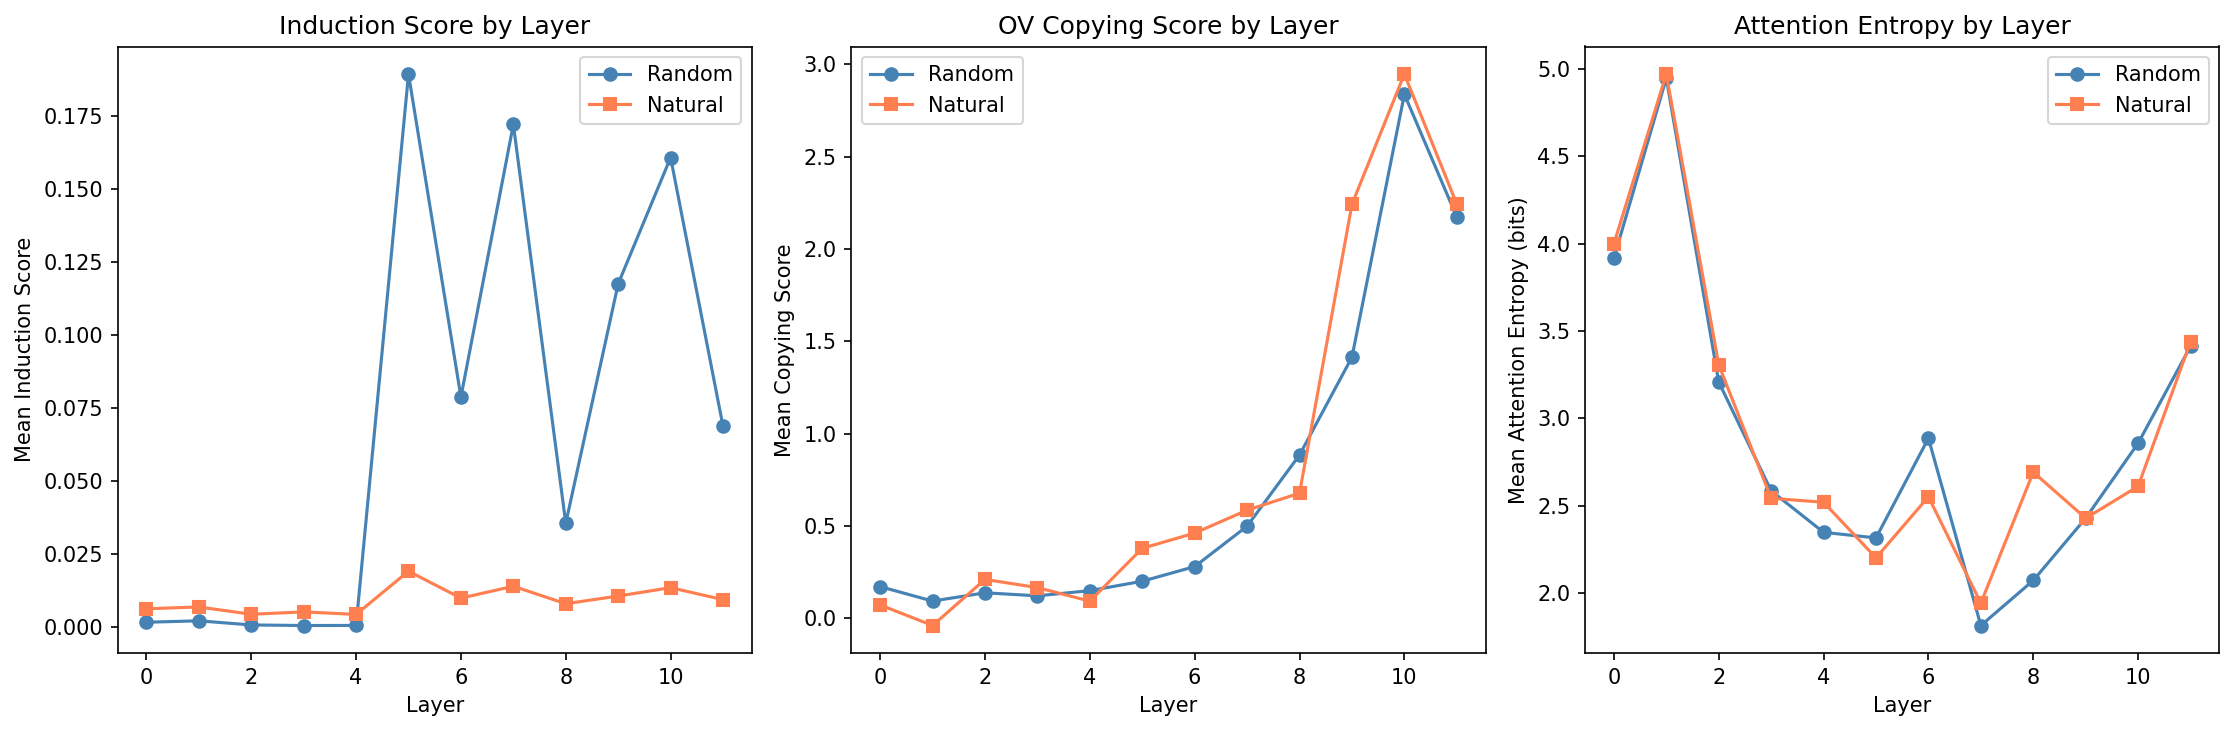
\includegraphics[width=0.95\linewidth]{figures/layer_analysis.png}
    \caption{Layer-wise analysis of induction scores, copying scores, and attention entropy. \figleft Induction scores diverge sharply (random $\gg$ natural) in layers 5--11. \figcenter Copying scores converge, with natural exceeding random in late layers. \figright Attention entropy is similar across conditions, indicating the score difference is not due to globally more diffuse attention.}
    \label{fig:layer}
\end{figure}

\subsection{Ablation Confirms Causal Importance}
\label{sec:results_ablation}

To verify that random-detected induction heads genuinely contribute to natural language processing, we zero out their attention patterns and measure the increase in next-token prediction loss on \owt passages (\figref{fig:ablation}).

\begin{figure}[t]
    \centering
    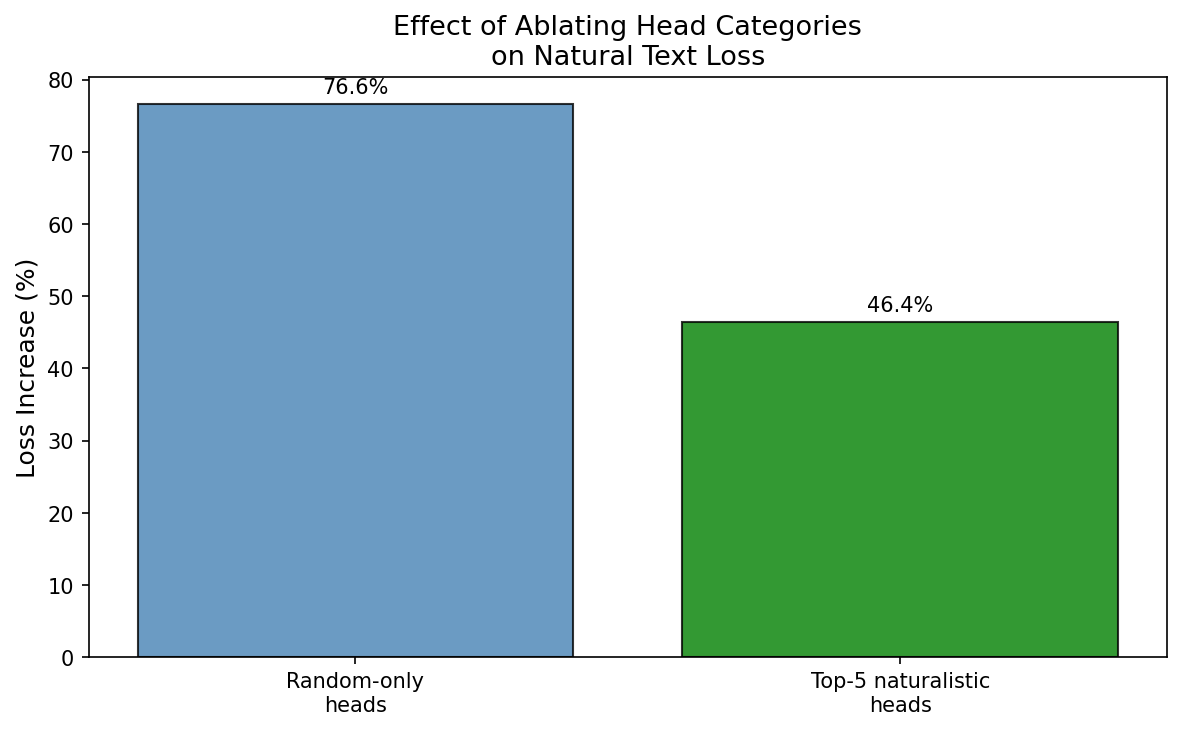
\includegraphics[width=0.65\linewidth]{figures/ablation_results.png}
    \caption{Ablation results on natural text. Removing the 21 random-detected induction heads (score $> 0.10$) increases loss by 76.6\%, while removing only the top-5 naturalistic-scoring heads increases loss by 46.4\%. These heads are not random-sequence specialists---they are causally important for natural language processing.}
    \label{fig:ablation}
\end{figure}

\Tabref{tab:ablation} summarizes the results.
Ablating all 21 random-detected heads increases loss from 3.047 to 5.380 ($+76.6\%$).
Even ablating only the 5 heads with the highest naturalistic induction scores increases loss by 46.4\%, confirming that these heads are not random-sequence specialists---they play a genuine role in natural language modeling, despite their low induction scores on natural text.

\begin{table}[t]
    \centering
    \caption{Ablation results on \owt passages. Both head groups substantially increase loss when removed, confirming their causal importance for natural language processing.}
    \label{tab:ablation}
    \begin{tabular}{@{}lccc@{}}
        \toprule
        Ablated Group & $N$ Heads & Ablated Loss & Loss Increase \\
        \midrule
        None (baseline)          & 0  & 3.047 & --- \\
        Random-detected ($\iscore > 0.10$) & 21 & 5.380 & \textbf{+76.6\%} \\
        Top-5 by natural $\iscore$   & 5  & 4.461 & +46.4\% \\
        \bottomrule
    \end{tabular}
\end{table}
